\documentclass{article}
\usepackage{ctex}
\usepackage[a4paper, total={6in, 8in}]{geometry}
\setlength{\parindent}{0pt}
\usepackage{amsmath,amssymb,amsfonts,color}
\usepackage{bm}
\usepackage{graphicx}
\usepackage{float} 
\usepackage{caption} 
\usepackage{subfigure}
\usepackage{algorithm}
\usepackage[document]{ragged2e}
\usepackage{xcolor}
\usepackage{setspace}
\usepackage{listings}
\setstretch{1.8}
\setlength{\parindent}{2em}
\begin{document}
{\centering\section*{优化方法第四章作业}}
\textcolor{blue}{1.总结等式约束凸优化问题的求解方法及相互联系}\\
1.解:\\
对于等式限制凸优化问题:\\
$min f(x)$\\
$s.t. Ax = b$\\
1.消除方法:消除等式约束,转化为等价的无约束问题\\
仿射可行解集$\{x|Ax = b\} = \{Fz + \hat{x} | z \in \mathbb{R}^{n-p}\} where \hat{x}$是满足$A\hat{x} = b$的任意特解\\
消除矩阵$F \in \mathbb{R}^{n x (n-p)}$是值域$R(F)$为A的零空间的任意矩阵\\
消除等式约束后的优化问题:$\min\limits_{z\in\mathbb{R}^{n-p}} \hat{f}(Fz + \hat{x}) \Leftrightarrow min\{f(x) | s.t.Ax = b\}$\\
最优解$z^*$确定原等式约束问题的最优解$x^* = Fz^* + \hat{x}$\\
牛顿方向:$d_z = -(\nabla ^2 \widetilde{f}(z))^{-1} \nabla \widetilde{f}(z) = -(F^T\nabla^2f(x)F)^{-1}F^T\nabla f(x)$\\
\textcolor{red}{与对偶函数联系:$Fd_z = d_x,\hat{f}$在z处的牛顿减少量$\hat{\lambda}(z)$与f在x处的牛顿减少量$\lambda(x)$相等}\\

2.对偶方法:采用无约束优化方法求解对偶问题,然后从对偶问题中复原等式约束优化问题的解\\
对偶函数:$g(v) = -b^Tv + \inf\limits_x (f(x) + v^TAx) = -b^Tv - \sup\limits_x((-A^Tv)^Tx - f(x)) = -b^Tv- f^*(-A^Tv)$\\
对偶问题:$\max\limits_x -b^Tv- f^*(-A^Tv)$该问题存在最优解,Slater条件满足,从而强对偶性成立,故$g(v^*) = p^*$\\
这样就将问题转化为了无约束最优化问题:\\
$\min\limits_x f(x) + (v^*)^T(Ax-b) \Leftrightarrow \nabla f(x) + A^Tv^* = 0$\\
$s.t. A(x+v) = b$\\
故$v^* = - (AA^T)^{-1}A\nabla f(x^*)$为原等式约束问题的一个最优对偶变量\\
采用无约束凸优化问题牛顿方法求解\\
目标函数$f(x)$在$x$附近的二阶Taylor近似模型:
$\min\limits_v \hat{f}(x+v) = f(x) + \nabla f(x)^Tv + \frac{1}{2}v^T\nabla ^2f(x)v$\\
$Ax^* - b, \nabla f(x^*) + A^Tv^* = 0$,因为$x^* = x + d_x, v^* = w$故\\
$Ad_x = 0, \nabla^2 f(x)d_x + A^Tw = -\nabla f(x)$即
$$
\begin{gathered}
    \left[
        \begin{array}{cccc}
            \nabla ^2f(x) & A^T \\
            A & 0
        \end{array} 
    \right]
    \left[
        \begin{array}{cccc}
            d_x \\
            w
        \end{array} 
    \right]
    $=$
    \left[
        \begin{array}{cccc}
            -\nabla f(x)\\
            0 
        \end{array}
    \right]
\end{gathered}
$$\\
$d_x$为x处的牛顿方向\\
等式约束优化问题牛顿减少量$\lambda(x) = (d_x^T \nabla^2 f(x) d_x)^{\frac{1}{2}}$\\
函数f在x处的二次展开$\hat{f}(x+v) = f(x) + \nabla f(x)^T v + \frac{1}{2}v^T \nabla^2 f(x)v$\\
$f(x) - p^* \approx f(x) - inf(\hat{f}(x+v):A(x+v) = b) = \frac{1}{2}(\lambda(x))^2$\\
$f$沿着$d_x$的方向导数:$-\lambda(x)^2$\\
等式约束的牛顿方法:\\
\textcolor{red}{
初始化可行点$x^0,Ax^0 = b$,\\
确定牛顿方向和牛顿减少量:
$$
\begin{gathered}
    \left[
        \begin{array}{cccc}
            \nabla ^2f(x) & A^T \\
            A & 0
        \end{array} 
    \right]
    \left[
        \begin{array}{cccc}
            d_x \\
            w
        \end{array} 
    \right]
    $=$
    \left[
        \begin{array}{cccc}
            -\nabla f(x)\\
            0 
        \end{array}
    \right]
\end{gathered}
$$
$\lambda(x)^2 = d_x^T \nabla^2 f(x) d_x$\\
停止准则$\frac{1}{2}\lambda(x^k)^2 \leq \epsilon$\\
回溯直线搜索$0<\alpha<0.5,0<\beta<1,t^k = 1$\\
$while( f(x^k + t^kd^k_x) > f(x^k) + \alpha t^k \nabla f(x^k)^T d^k_x = f(x^k) - \alpha t^k \lambda(x^k)^2)$\\
$t^k = \beta t^k$}\\
不可行初始点的牛顿方向:\\
找到一个在当前不可行点出牛顿方向$d$使得$x+d$近似满足最优性条件,即$x + d \approx x^*$\\
由$Ax^* = b, \nabla f(x^*) + A^Tv^* = 0$得 $A(x+d) = b,\nabla f(x^*) + \nabla f^2(x)d + A^Tw = 0$\\
即$$
\begin{gathered}
    \left[
        \begin{array}{cccc}
            \nabla ^2f(x) & A^T \\
            A & 0
        \end{array} 
    \right]
    \left[
        \begin{array}{cccc}
            d \\
            w
        \end{array} 
    \right]
    $=$-
    \left[
        \begin{array}{cccc}
            \nabla f(x)\\
            Ax-b
        \end{array}
    \right]
\end{gathered}
$$\\
原对偶残差:\\
$$\begin{gathered}
    Let \quad y = \left[
        \begin{array}{cccc}
            x\\
            v 
        \end{array} 
    \right]\\
    Then \quad r(y) = \left[
        \begin{array}{cccc}
            \nabla f(x) + A^Tv\\
            Ax - b
        \end{array} 
    \right]
    \triangleq
    \left[
        \begin{array}{cccc}
            r_{dual}(y)\\
            r_{pri}(y)
        \end{array} 
    \right]
\end{gathered}
$$\\
这样,原等式约束凸优化问题优化过程等价于:给定任意$y$,找到一个下降方向$d_y$,使得$y + d_y$满足最优性条件,即$r(y+ d_y) = 0$\\
原对偶残差在当前估计点y附近的一阶$Taylor$近似为:$r(y+z) \approx r(y) + Dr(y)z$
$$\begin{gathered}
    Dr(y) = \left[
        \begin{array}{cccc}
            \nabla^2 f(x) & A^T\\
            A & 0 
        \end{array} 
    \right]\\
\end{gathered}
$$\\
$r(y) + Dr(y)dy = 0 \Rightarrow $
$$\begin{gathered}
    \left[
        \begin{array}{cccc}
            \nabla^2 f(x) & A^T\\
            A & 0 
        \end{array} 
    \right]
    \left[
        \begin{array}{cccc}
            d_x\\
            d_v 
        \end{array} 
    \right]
    =\quad -
    \left[
        \begin{array}{cccc}
            \nabla f(x)  + A^Tv\\
            Ax-b
        \end{array} 
    \right]\\
\end{gathered}
$$\\
于是有:$d_y = -Dr(y)^{-1}r(y)$\\
不可行初始点的牛顿方向
$$
\begin{gathered}
    \left[
        \begin{array}{cccc}
            d\\
            w 
        \end{array} 
    \right]
    = 
    \left[
        \begin{array}{cccc}
            d_x\\
            v + d_v
        \end{array} 
    \right]
\end{gathered}
$$

不可行初始点牛顿下降回溯直线搜索方法:\\
\textcolor{red}{
初始化可行点$x^0 \in domf,v^0$,\\
停止准则$Ax^k = b \quad and \quad \Vert r(x^k,v^k) \Vert_2  \leq \epsilon$\\
确定原对偶牛顿方向:
$$
\begin{gathered}
    \left[
        \begin{array}{cccc}
            \nabla ^2f(x) & A^T \\
            A & 0
        \end{array} 
    \right]
    \left[
        \begin{array}{cccc}
            d_x^k \\
            d_v^k
        \end{array} 
    \right]
    $=$\quad - 
    \left[
        \begin{array}{cccc}
            -\nabla f(x^k) + A^T v^k\\
            Ax^k - b
        \end{array}
    \right]
\end{gathered}
$$
对原对偶残差$\Vert r \Vert_2$进行回溯,确定步长$t^k$\\
$while( \Vert r(x^k+t^kd^k_x, v^k + t^kd^k_v) \Vert_2 > (1-\alpha t^k) \Vert r(x^k,v^k) \Vert_2)$\\
$t^k = \beta t^k$\\
$x^{k+1} = x^k + t^kd^k_x, v^{k+1} = v^k + t^kd^k_v$返回检测停止准则}\\
为止初始点牛顿方法的收敛性分析:\\
阻尼牛顿阶段:$\Vert r(y^k)\Vert_2 > \frac{1}{K^2L}, \quad \Vert r(y + td_y) \Vert_2 \leq (1 - \alpha t)\Vert r(y)\Vert_2$\\
二次收敛阶段:$\Vert r(y^k)\Vert_2 \leq \frac{1}{K^2L},\quad \frac{K^2L\Vert r(y^{l+k})\Vert_2}{2} \leq (\frac{K^2L\Vert r(y^{l})\Vert_2}{2})^{2^k} \leq (\frac{1}{2})^{2^{k}}$

\newpage
\textcolor{blue}{2.等式约束熵极大化\\
等式约束熵极大化问题:$min f(x) = \sum_{i = 1}^{n}x_ilogx_i$\\
subjected to $Ax = b_i$\\
采用以下方法计算该问题的解:\\
(a)标准Newton方法:}\\

\begin{figure}[H] 
    \centering 
    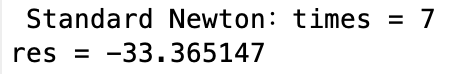
\includegraphics[width=0.6\textwidth]{Newtonres1.png}
\end{figure}
以$log(f(x^k) - p^*)$为纵轴,$k$为横轴画图:\\
\begin{figure}[H] 
    \centering 
    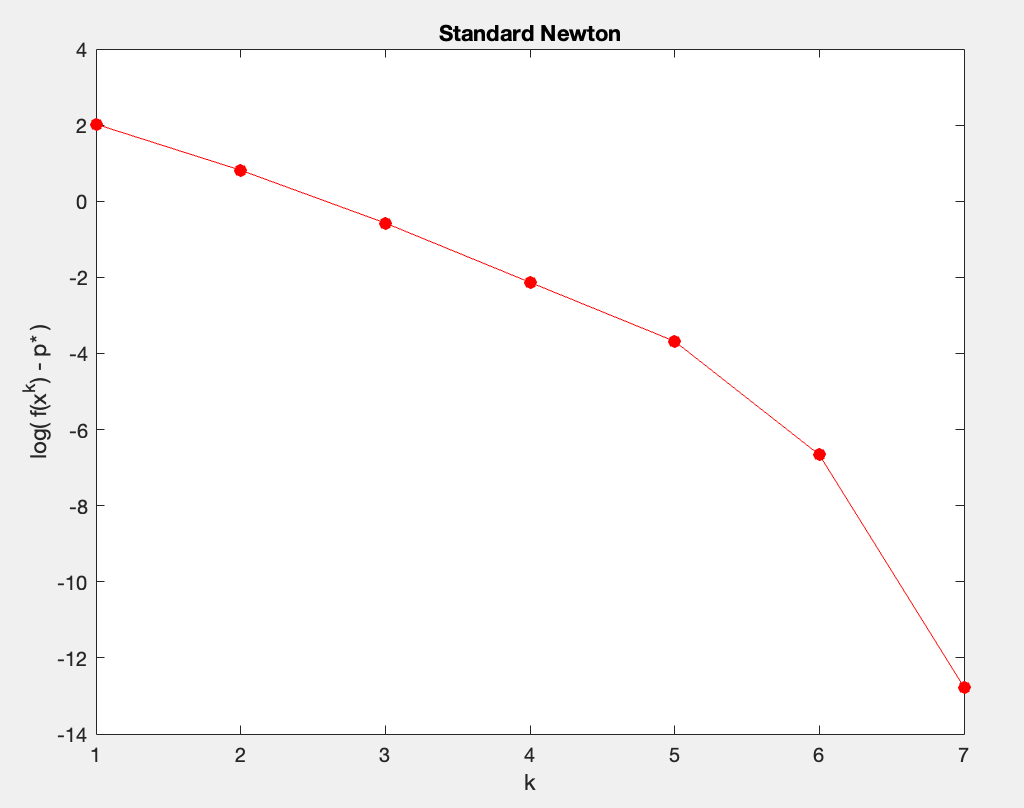
\includegraphics[width=0.8\textwidth]{Newtonfig1.png}
\end{figure}

\textcolor{blue}{(b)不可行初始点Newton方法:}\\
\begin{figure}[H] 
    \centering 
    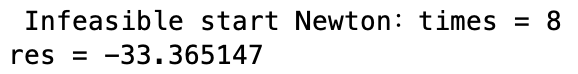
\includegraphics[width=0.6\textwidth]{Newtonres2.png}
\end{figure}
以$log(f(x^k) - p^*)$为纵轴,$k$为横轴画图:
\begin{figure}[H] 
    \centering 
    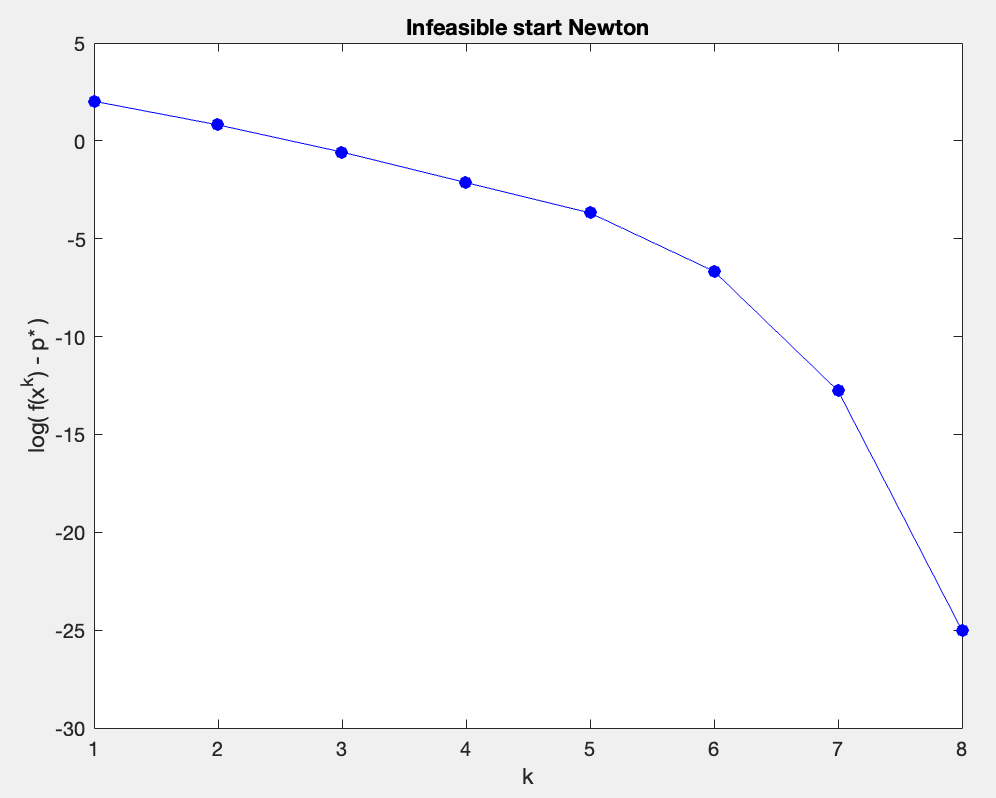
\includegraphics[width=0.8\textwidth]{Newtonfig2.png}
\end{figure}

\textcolor{blue}{(c)对偶newton方法:}\\

\begin{figure}[H] 
    \centering 
    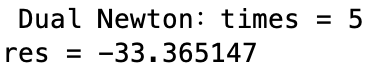
\includegraphics[width=0.6\textwidth]{Newtonres3.png}
\end{figure}
以$log(L(v^k) - d^*)$为纵轴,$k$为横轴画图:
\begin{figure}[H] 
    \centering 
    \includegraphics[width=0.8\textwidth]{Newtonfig3.png}
\end{figure}
由代码输出及图像得,起始点相同时,三种方法的结果相同。\\
在标准牛顿方法和不可信初始点牛顿方法中,计算系数矩阵
$$
\begin{gathered}
    \left[
        \begin{array}{cccc}
            \nabla ^2f(x) & A^T \\
            A & 0
        \end{array} 
    \right]
\end{gathered}
$$
来解决问题。其中$\nabla ^2f(x) = \textbf{diag}(x)^{-1}$\\ 
这样系数矩阵就可以表示为$A\textbf{diag}(x)A^T$\\
在对偶牛顿方法中,计算系数矩阵$-\nabla ^2 g(v) = ADA^T$,这里$D_{ii} = e^{-a^T_i v - 1}$\\



\end{document}